\section{Artifact removal}\label{sec1}

Nuclear magnetic resonance (NMR) spectroscopy has the ability to select discrete region within the body for signal acquisition \cite{13}. A radio frequency (RF) pulse presses the protons thus producing a free induction decay (FID) signal as in figure \ref{1}. This signal contains a lot of information regarding the metabolite activity in the region of interest (ROI). Since a human body mostly contains of water, thus, the water peak on the MRS spectrum has a much higher amplitude compare to the other metabolites \ref{2}. In order to observe the quantity of the rest of metabolites it is important to remove the water frequency component without distortion of the rest of the spectrum. 

\begin{figure}[!htbp]
\minipage{0.5\textwidth}%
\centering
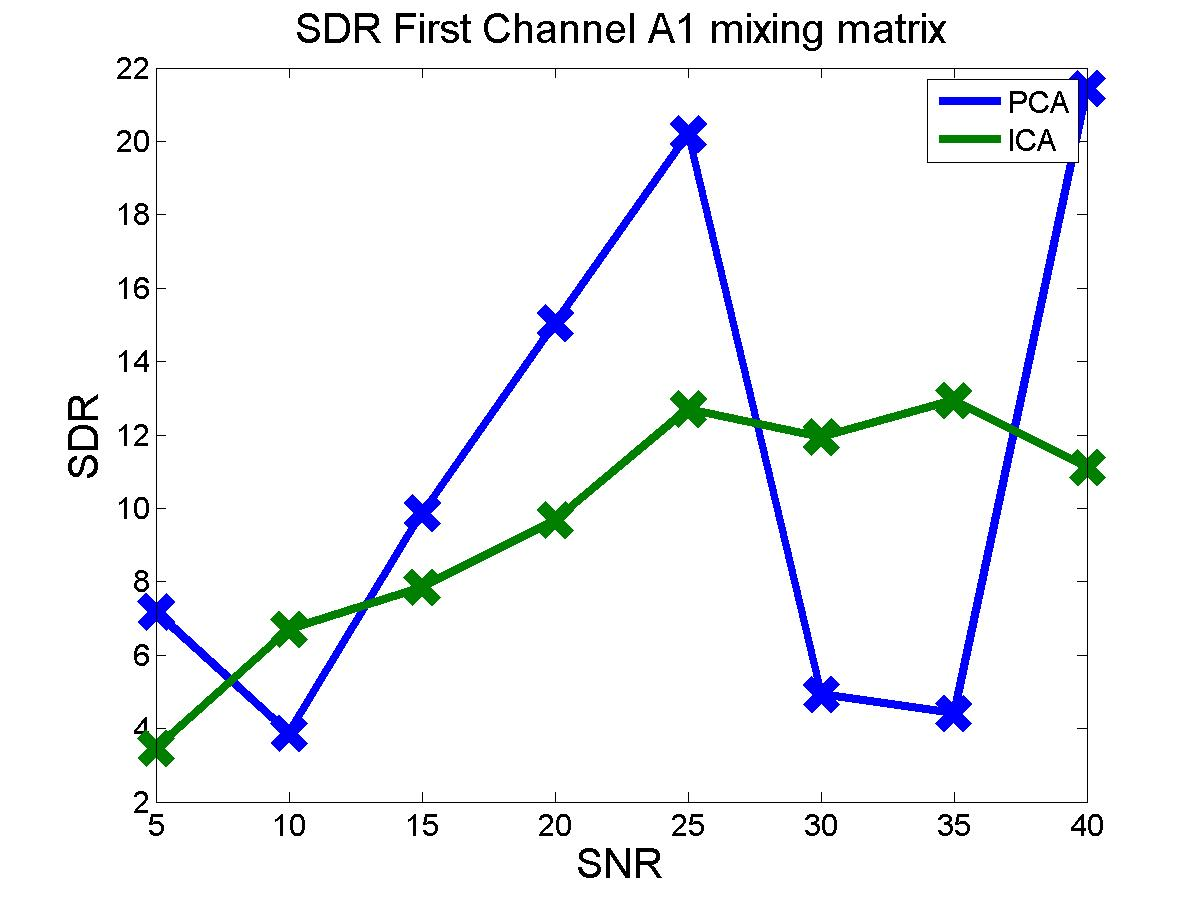
\includegraphics[width=0.7\textwidth]{1.jpg}
\subcaption{NMR signal in time domain}\label{1}
\endminipage\hfill
\minipage{0.5\textwidth}%
\centering
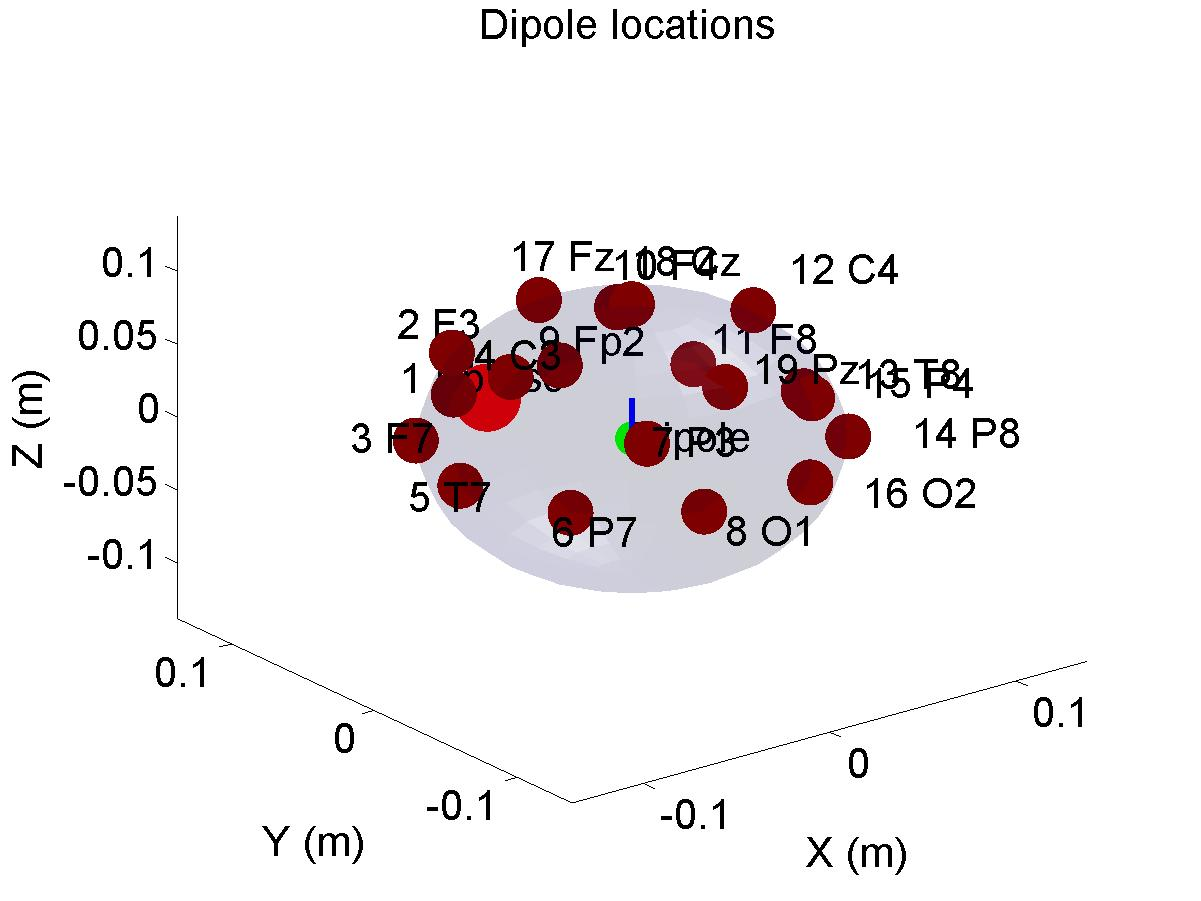
\includegraphics[width=0.7\textwidth]{2.jpg}
\subcaption{NMR Spectrum of the signal in ppm}\label{2}
\endminipage\hfill
\caption{The raw signal acquired from the MRS }
\end{figure}

Water peaks on the NMR spectrum are considered to be an artifact and their suppression is achieved by omitting the decomposed component where their central frequencies is higher than $4.7 ppm$. This components has to be deduced from the original signal, whereby the rest of the desired metabolites will become more pronounced. 

\begin{figure}[!htbp]
\centering
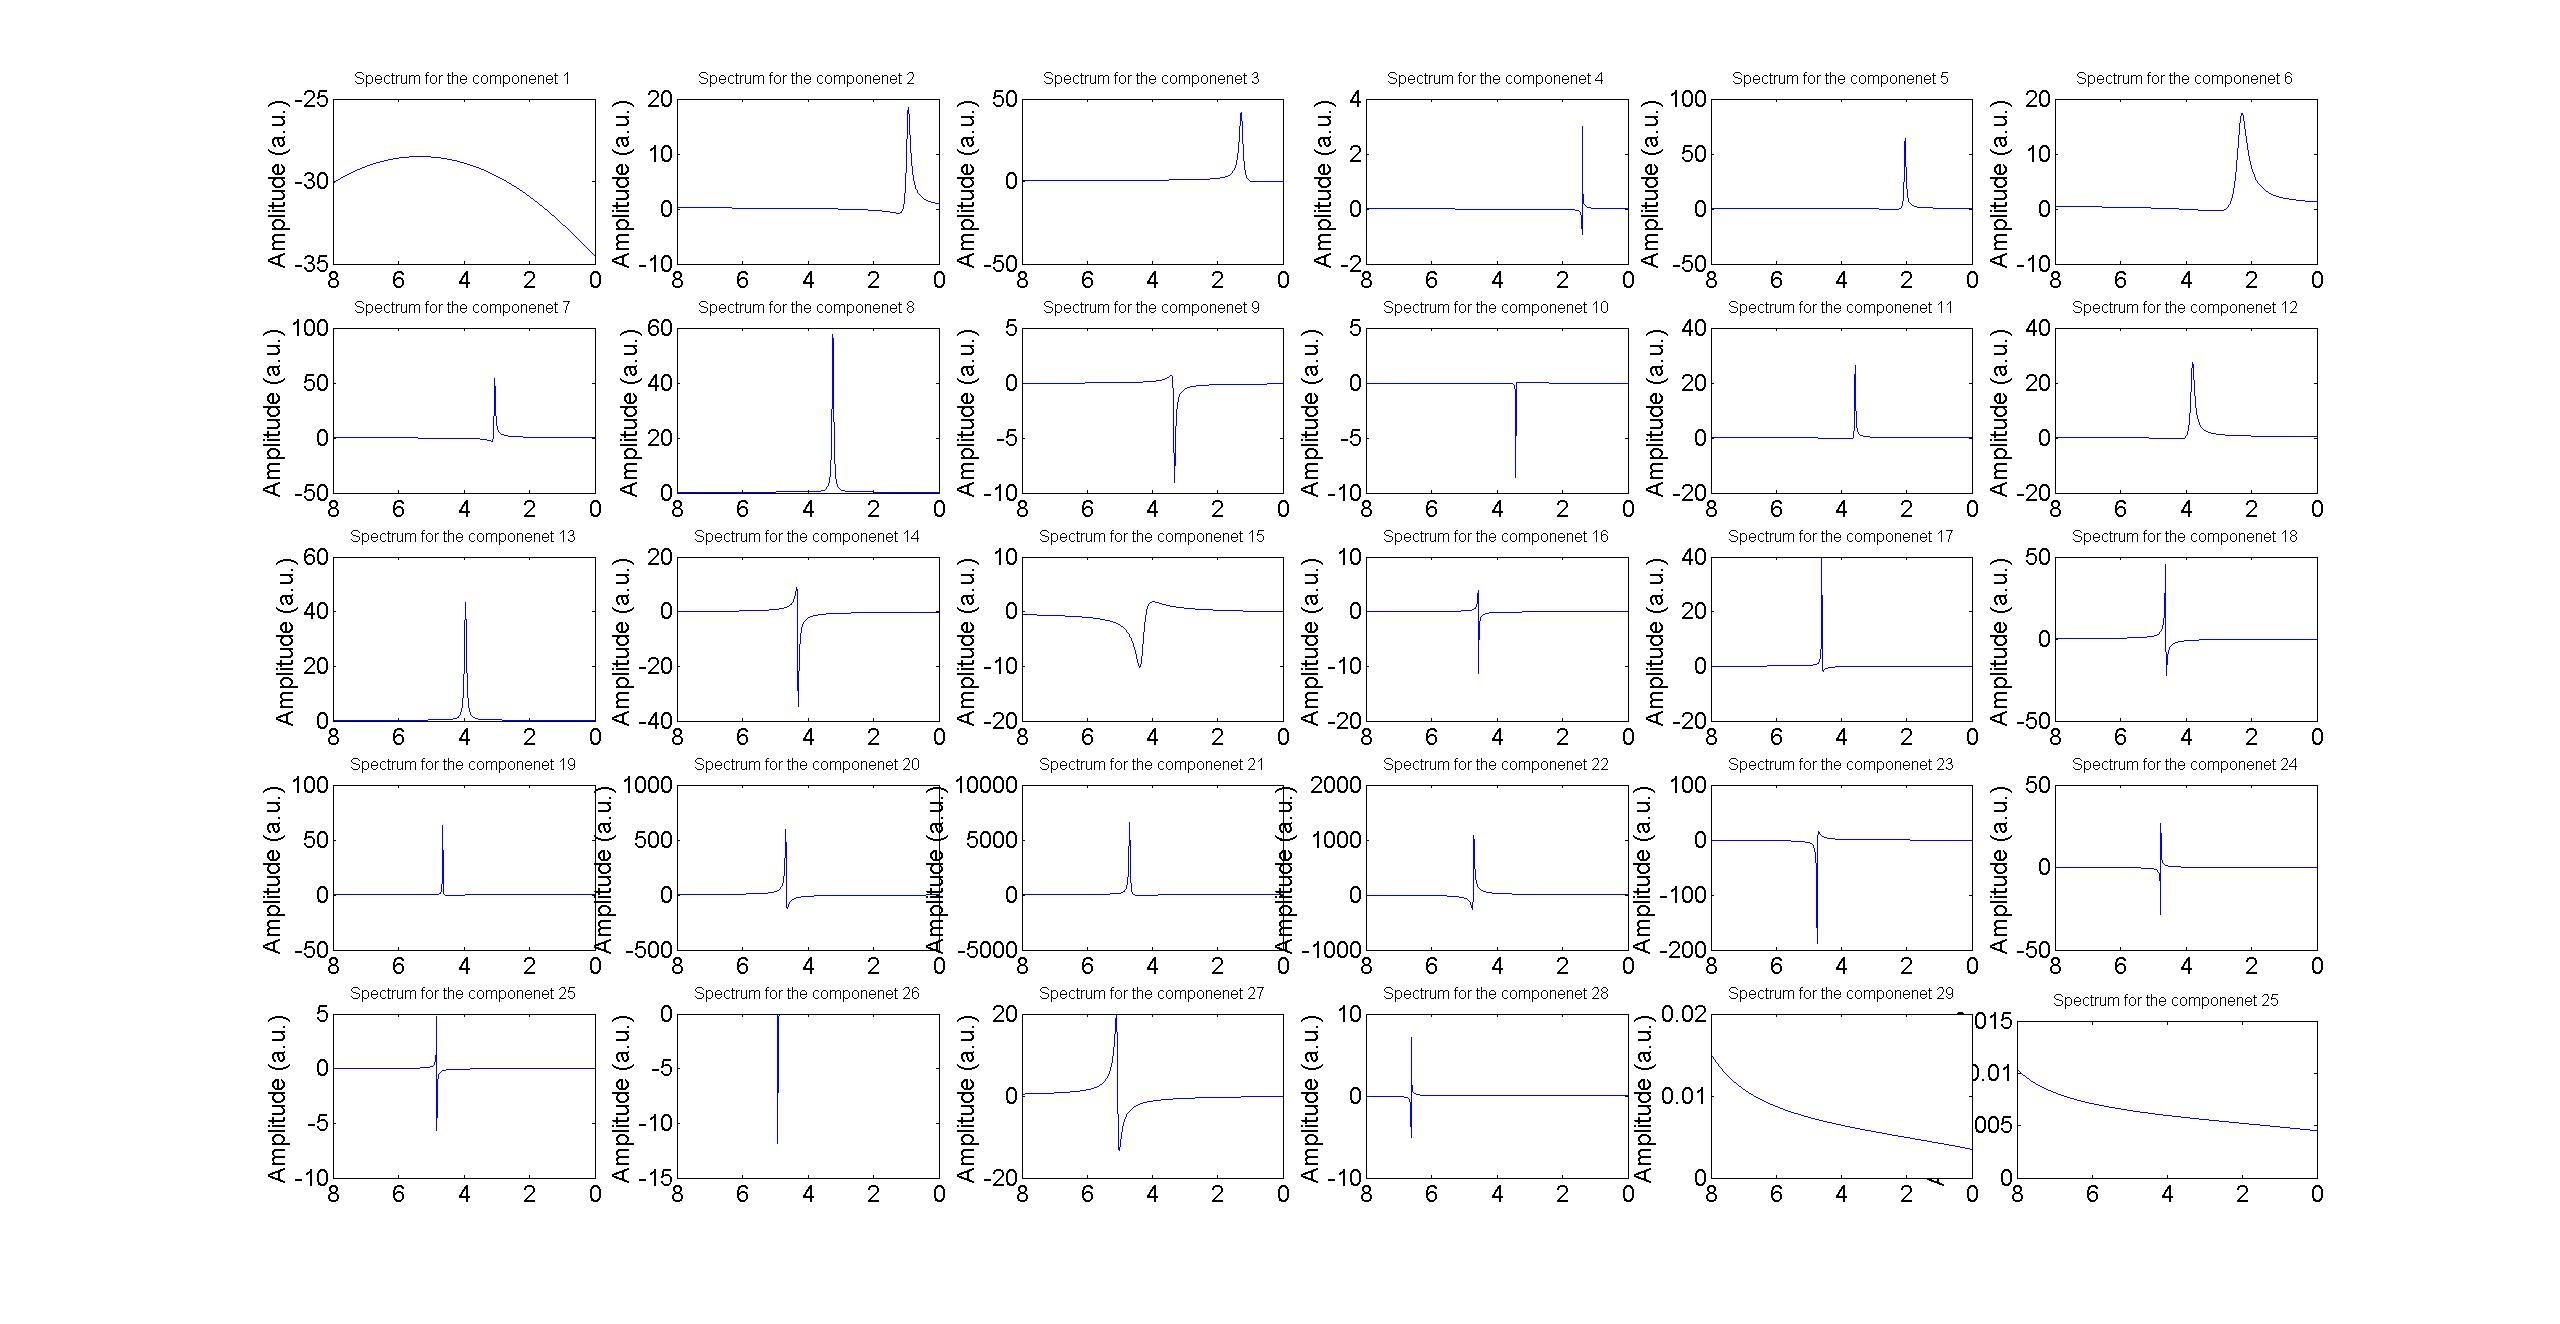
\includegraphics[width=0.8\textwidth]{IndividualComponents.jpg}
\caption{ Individual components ordered on by the central frequency.}
\end{figure}

Hereby it is also very important to define the model order of the decomposition for high performance of artifact suppression. Two models order selection are being investigated. Minimum description length (MDL) and rank determination are two eligible methods for model order selection \cite{21}.In figures \ref{3} and \ref{4} is the performance graph for MDL and rank determination method respectively. MDL indicates that that the higher the model order the better the performance of filtering and a similar result is provided from the rank determination. 


\begin{figure}[!htbp]
\minipage{0.5\textwidth}%
\centering
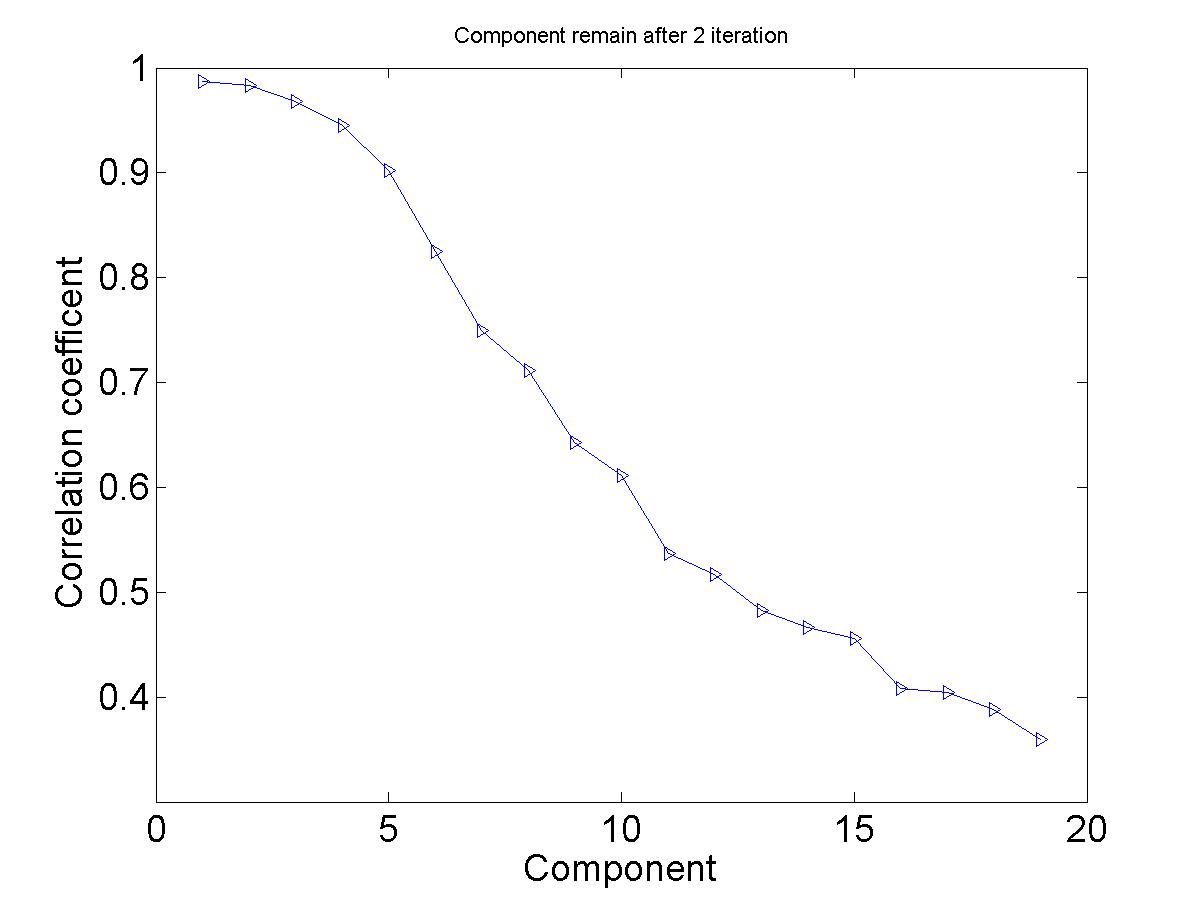
\includegraphics[width=0.7\textwidth]{39.jpg}
\subcaption{Rank determination outcome}\label{3}
\endminipage\hfill
\minipage{0.5\textwidth}%
\centering
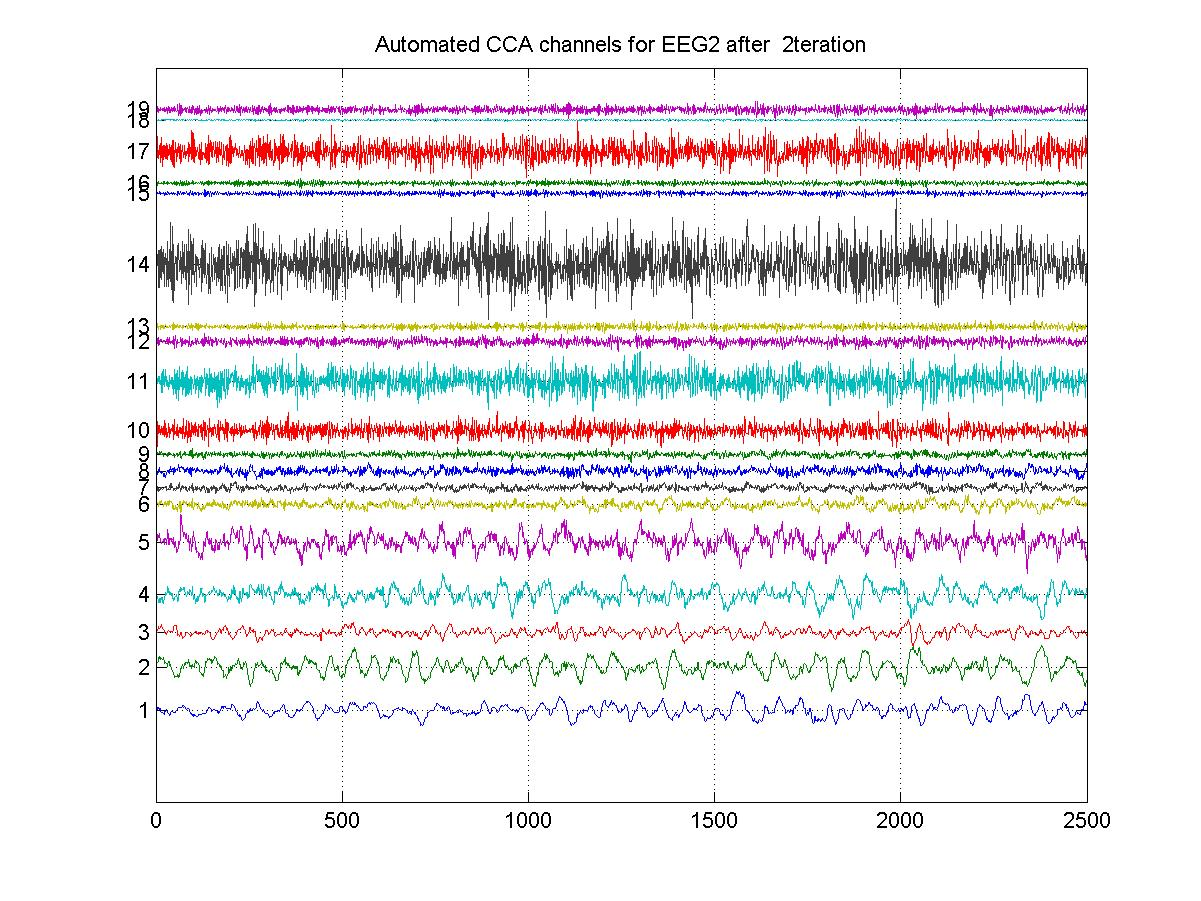
\includegraphics[width=0.7\textwidth]{40.jpg}
\subcaption{MDL outcome}\label{4}
\endminipage\hfill
\caption{Model order selection}\label{5}
\end{figure}

A reasonable model order is necessary since underestimated model might omit the necessary pics needed to be suppressed. On the other hand, a very large order could generate unwanted spectrum including noise component \cite{1}. In this case we have selected a model order of 29 since the it is a good moderation with the low processing complexity and the high performance.

The final signal for different model order could be found in \ref{A1}. Whereas the filtered signal for the model order that suits the best for the implementation is in figure \ref{3} with the water signal to be filtered out in the figure \ref{4}.
The frame length luckily is much larger than the order of the signal model, therefore the correlation to be embedded could be fully explored\cite{2}. 


Regarding the dimension $(LxM)$ of the Hankel matrix ($H$),a high number of rows ($L$) is required, given the orthogonality of signal ($\hat{H}$) and noise ($W$). This is on the beneficial to the noise removal from the approximation $\hat{H}W\approx 0$. This last approximation in practice is not easy to be achieved, however, it approaches more and more to with the over-determination of the system. Therefore a $L>>M$ is necessary. However it has to be compromised with number of columns $M$, otherwise, a very large number of rows will reduce the number of columns being introduced. Therefore, this will worsen the approximation $H_{n}^{T}H_{n}\approx\sigma_{v}^2I$ \cite{11}. The best performance and accuracy of the system is obtained when the Hankel matrix is a rectangular case. This will speed up the processing time of the Karhunen–Loève Transform (KLT) and it compromises the number of rows and the number of columns.


\begin{figure}[!htbp]
\minipage{0.5\textwidth}%
\centering
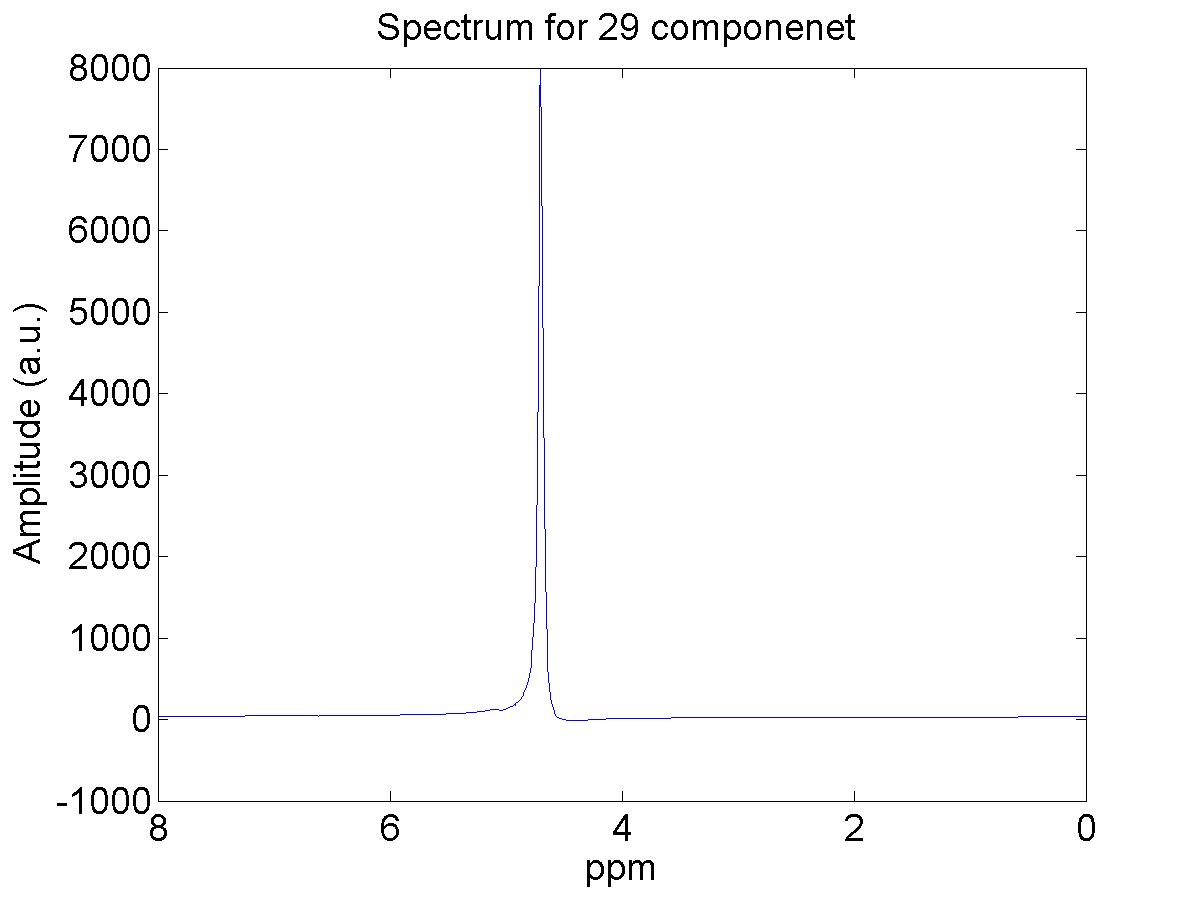
\includegraphics[width=0.7\textwidth]{27.jpg}
\subcaption{Water component}\label{3}
\endminipage\hfill
\minipage{0.5\textwidth}%
\centering
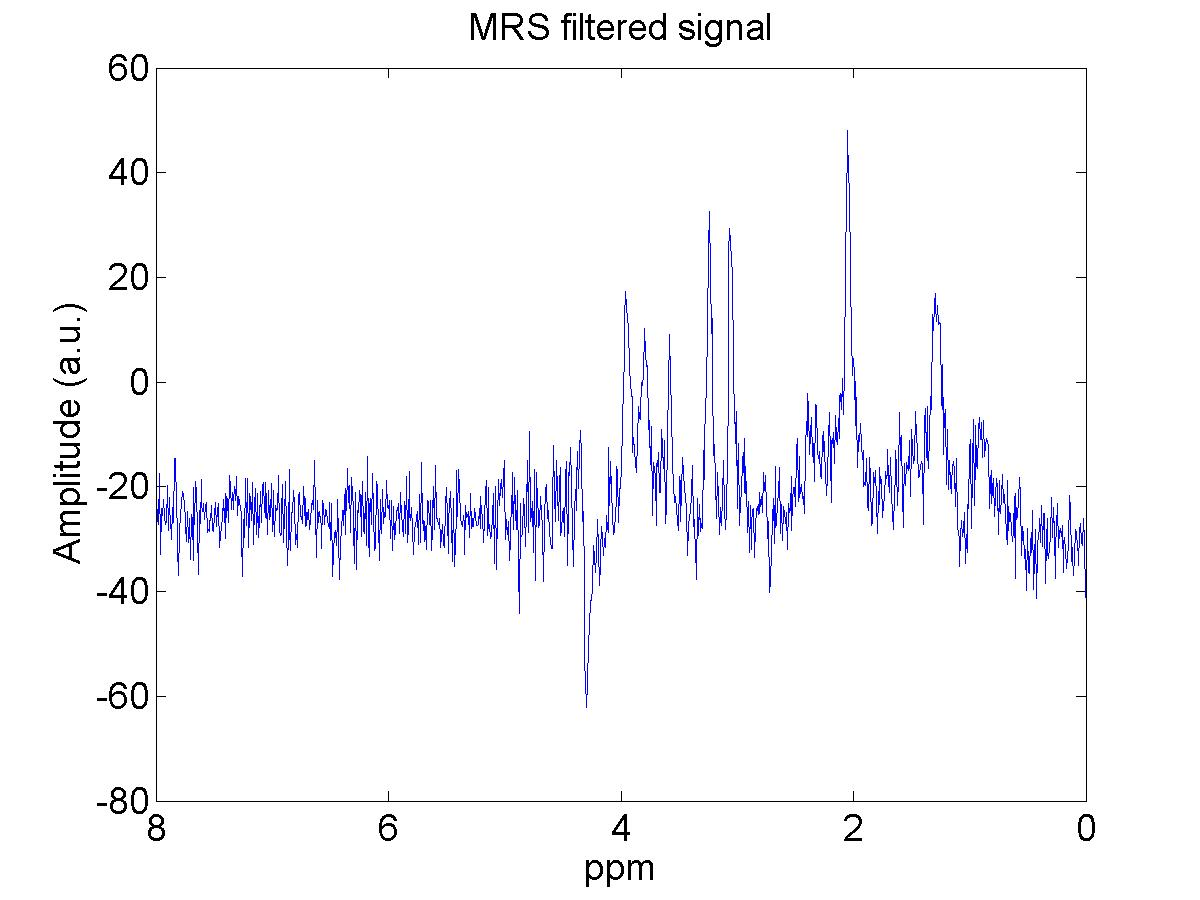
\includegraphics[width=0.7\textwidth]{28.jpg}
\subcaption{Water filtered signal}\label{4}
\endminipage\hfill
\caption{Final results}\label{5}
\end{figure}

The water filtering is done by removing the water component in figure \ref{3} from the original signal spectrum in figure \ref{2}. 

\subsection{Comparison with classical filters}

\begin{itemize}


\item The superior benefit of subspace filtering consists in its ability to recover the clean signal with the minimum distortion as well as the minim residue noise possible. In spectral based and Wiener filtering approach, the noise removal is a process which also introduces distortion to the wanted signal. This obstacle is overcomed in subspace methods by nulling the noisy subspace which has no mutual information with other desired subspaces. Additionally, the noise accumulated in the subspace to be nulled is on higher amount compare to amount of noise being suppressed via the spectral methods \cite{3}. 

\item Spectral based method is restricted by a fixed Fast Fourier Transform (FFT) computing whereas Singular Value Decomposition (SVD) based topologies vary in computational time with the KLT data. In addition, KLT transform $O(nm^2)$ is far more heavy in terms of computation time compare to FFT $O(nlog(n))$ \cite{2}.

\item Moreover, in this content subspace methods assume explicitly the order of the signal, or in other word the rank-deficient speech observation matrix. Whereas Wiener filtering does an implicit rank reduction based on a estimation of rank reduced correlation matrix \cite{2}.

\item Apart from the FFT spectral based, Discrete cosine transform (DCT) is another candidate for signal enhancement. Yet it is far superior compare to the theoretical subspace filtering\cite{2}.

\item Differently from the classical filters, subspace methods efficiency depend significantly on the ability of the user to identify the accuracy of the characteristics of the underlying signal. The better the properties are defined the better the removal of the noises is performed\cite{5}. The other classical filters require no need of any additional visualization skills, therefore, are mostly applied in fully automated framework.

\item In order to consistently apply the subspace filtering, the signal has to be modelled into a clear analytical formulation. In some modalities this is not a very easy task consequently its application is restricted into very well known physical models.

\item Another fundamental issue with subspaces signal is that noise incorporated in the signal which needs to be reduced is considered white. In case of narrow band noises a pre-whitening step has to be applied before the filtering itself takes place, given the noise covariance matrix is known \cite{6}.

\end{itemize}
